\documentclass[tikz,border=2mm]{standalone}
\usepackage{pgfplots}
\pgfplotsset{compat=1.17}
\usepgfplotslibrary{groupplots}
\begin{document}
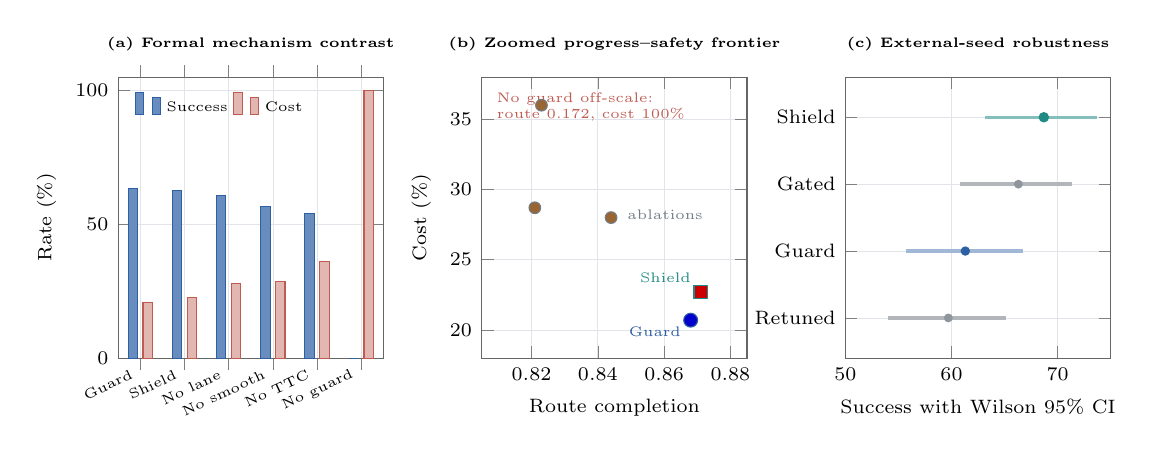
\begin{tikzpicture}
\definecolor{oursblue}{RGB}{45,95,163}
\definecolor{oursgreen}{RGB}{32,139,132}
\definecolor{costred}{RGB}{190,92,82}
\definecolor{neutral}{RGB}{115,123,132}
\definecolor{lightgrid}{RGB}{225,228,232}
\begin{groupplot}[
  group style={group size=3 by 1, horizontal sep=1.25cm},
  width=4.95cm,
  height=5.15cm,
  tick label style={font=\scriptsize},
  label style={font=\scriptsize},
  title style={font=\tiny\bfseries},
  legend style={font=\tiny, draw=none, fill=none},
  grid=major,
  major grid style={draw=lightgrid,line width=0.25pt},
  axis line style={black!60},
]
\nextgroupplot[
  title={(a) Formal mechanism contrast},
  ybar,
  bar width=3.4pt,
  ymin=0,ymax=105,
  ylabel={Rate (\%)},
  symbolic x coords={Guard,Shield,No lane,No smooth,No TTC,No guard},
  xtick=data,
  xticklabels={Guard,Shield,No lane,No smooth,No TTC,No guard},
  x tick label style={font=\tiny, rotate=25, anchor=east},
  legend columns=2,
  legend pos=north west,
]
\addplot+[draw=oursblue,fill=oursblue!72] coordinates {(Guard,63.3) (Shield,62.7) (No lane,60.7) (No smooth,56.7) (No TTC,54.0) (No guard,0.0)};
\addlegendentry{Success}
\addplot+[draw=costred,fill=costred!45] coordinates {(Guard,20.7) (Shield,22.7) (No lane,28.0) (No smooth,28.7) (No TTC,36.0) (No guard,100.0)};
\addlegendentry{Cost}

\nextgroupplot[
  title={(b) Zoomed progress--safety frontier},
  xlabel={Route completion},
  ylabel={Cost (\%)},
  xmin=0.805,xmax=0.885,
  ymin=18,ymax=38,
]
\addplot+[only marks,mark=*,mark size=2.5pt,draw=oursblue,fill=oursblue] coordinates {(0.868,20.7)};
\node[font=\tiny,anchor=north east,text=oursblue] at (axis cs:0.868,20.9) {Guard};
\addplot+[only marks,mark=square*,mark size=2.4pt,draw=oursgreen,fill=oursgreen] coordinates {(0.871,22.7)};
\node[font=\tiny,anchor=south east,text=oursgreen] at (axis cs:0.871,22.7) {Shield};
\addplot+[only marks,mark=*,mark size=2.1pt,draw=neutral,fill=neutral!70] coordinates {(0.844,28.0) (0.821,28.7) (0.823,36.0)};
\node[font=\tiny,anchor=west,text=neutral] at (axis cs:0.846,28.2) {ablations};
\node[font=\tiny,anchor=north west,align=left,text=costred] at (rel axis cs:0.02,0.98) {No guard off-scale:\\route 0.172, cost 100\%};

\nextgroupplot[
  title={(c) External-seed robustness},
  xlabel={Success with Wilson 95\% CI},
  xmin=50,xmax=75,
  ymin=0.4,ymax=4.6,
  ytick={1,2,3,4},
  yticklabels={Retuned,Guard,Gated,Shield},
]
\draw[line width=1.2pt, color=neutral!55] (axis cs:54.0,1) -- (axis cs:65.1,1);
\fill[neutral!80] (axis cs:59.7,1) circle (1.6pt);
\draw[line width=1.2pt, color=oursblue!45] (axis cs:55.7,2) -- (axis cs:66.7,2);
\fill[oursblue] (axis cs:61.3,2) circle (1.7pt);
\draw[line width=1.2pt, color=neutral!55] (axis cs:60.8,3) -- (axis cs:71.4,3);
\fill[neutral!80] (axis cs:66.3,3) circle (1.6pt);
\draw[line width=1.2pt, color=oursgreen!55] (axis cs:63.2,4) -- (axis cs:73.7,4);
\fill[oursgreen] (axis cs:68.7,4) circle (1.9pt);
\end{groupplot}
\end{tikzpicture}
\end{document}
